%!TEX root = ../thesis.tex

\chapter{Introduction}\label{ch:introduction}

\section{History of natural gas in The Netherlands}

% Inleiding

%---------

% Geschiedenis

% stukje geschiedenis over gas in Groningen bel en Nederland.

%"De Nederlandse Aardolie Maatschappij heeft in haar exploratieboring bij Slochteren aardgas aangetroffen. Er zullen productieproeven worden genomen."
% Het Vrije Volk van 5 augustus 1959

% https://en.wikipedia.org/wiki/Groningen_gas_field
% Dutch disease
% https://en.wikipedia.org/wiki/Dutch_disease

% De huidige afhankelijkheid van gas: zie energie trends.
% Aardbevingen in groningen en protest tegen gas
% Aardbevingen laten zien: https://nl.wikipedia.org/wiki/Aardgasveld_van_Slochteren
% Klimaat problemen met de gas consumptie

% Regering wil over ~30 jaar van het gas af (vind source) (Parijs?)
% Dus huidige invrastructuur ligt er nog 30 jaar 
% Duur om te vervangen
% Hoe lang kunnen de leidingen blijven liggen, centrale vraag

%-----------

% stukje over voor wie we dit gaan doen.

% RUG
% Cogas
% valueA

%-----------

% Cathodic protection <-- eigen hoofdstuk

% Meetingen, en data grootte (wanneer was eerste meeting)

%----------

% Related work

%----------

% hypothese: wordt moeilijk om iets te zeggen over de lange termijn want er is weinig weinig data.


In 1959 on of the worlds largest natural gas deposit was found in Slochteren, The Netherlands \cite{nam-2014}. It was discovered by the "Nederlandse Aardolie maatschapij" (NAM)  which translates to: the Dutch oil Company. This company was founded by Shell and Esso in 1947 \cite{oprichting-nam} in order to find natural energy resources in the Dutch soil. The discovery of the natural gas deposit was kept with a low profile at first because Dutch law at that time \cite{mijnwet} did not give ownership of an natural occurring resource to its discoverer but to the state. After a follow up exploratory drilling near Delfzijl \todo{source} showed the size of the natural gas deposit \todo{how big} The NAM filed for the drilling rights with the Dutch Government for the Groningen area. 

Then in 1962 the Dutch government passed the natural gas bill \todo{cite}. It created a partnership between the Dutch state, Shell and Esso. The Dutch state would get a share of 50\%, Shell and Esso would both get a share of 25\%. The bill also founded the `Nederlandse Gasuni' (the Dutch union for natural gas). This union would be responsible for distributing the natural gas from the Slochteren field across the Netherlands. At that time there were local gas companies \todo{source} producing and distributing light gas distilled from coal. These companies would now distribute the Slochteren gas with their existing distribution network rather than produce their own.

In less than ten years most Dutch households would be connected with the gas network. The Netherlands would cook and be warmed by the Natural gas from Slochteren for foreseeable future. \todo{cite journaal wiki} The natural gas from Slochteren brought economical prosperity to The Netherlands in the second part of the 20th century. However there were also downsides. So much so that an economical term is named after it: `Dutch disease'. \todo{cite} This term is used when a nations products become expensive due to a strong currency, which is fueled by a newly discovered natural resource. Expensive exports causes a nations production to decrease and unemployment rates to rise.

\section{Current situation and future}

80 percent of the natural gas is thought to be extracted and at the current rate of extraction it is predicted that the gas will last for at-least another ten years. The gas is providing the Netherlands with warm homes and meals however the `mijnwet' gave ownership of the natural gas to the state. This meant that the revenues went the The Netherlands as a whole and not to directly to the regionals living directly on the gas field. Due to the extraction of the gas from the lower layers of the Earth, the upper layers start to shift with earthquakes as result. Because earthquakes are not common in The Netherlands, structures are not build to withstand their impact. This causes the houses of the residents directly above and near the gas field show signs of damages and sometimes become uninhabitable.

Without any direct benefit from the gas field but with their homes collapsing the people of Groningen started to oppose the extraction of the gas form the Slochteren field. Multiple protest groups have been formed over the years and not without success. The extraction of the natural gas will be limited from.. to .. a year. There have been made promises by the Dutch government to compromise the owners of damaged homes, however this is still to be implemented.

The earthquakes are not the only incentive for The Netherlands to stop extracting the gas. The Dutch government signed the Paris agreement in \todo{when}. The Paris agreement is a climate accord in which \todo{number of nations} made promises to reduce their carbon emissions in order to slow the global rising temperature. One of the promises The Netherlands made was to reduce the carbon emissions by ... percent. The Dutch government has stated that it wants to reduce the dependency on gas and start using other forms of energy instead. 

A third reason to reduce the dependency on gas is when the gas eventually runs out, the Netherlands will have to rely on importing gas from foreign nations such as Russia. Which can have undesirable consequences since Russia has been known to use their gas supplies as diplomatic leverage \todo{find source}.

For these three reasons The Netherlands is moving away from fossil fuels and transitioning to sustainable energy sources like wind and solar power. The transition to `green' energy will take time. The energy infrastructure needs to be able to handle a bigger dependency on electricity and facilities need to be build to produce the electricity. During this time the current gas infrastructure will still be in use.


The gas infrastructure or transition systems in The Netherlands are hold by operator companies (TSOs). There are seven TSOs in The Netherlands facilitating the 7.6 \todo{energie trends} million Dutch households. These TSOs maintain and expand their infrastructure. 

Replacing broken pipe infrastructure is a large expenditure for the TSOs, in 2014 together the TSOs spend 679 billion euro \todo{source energy trends} in replacing and maintaining the current transition systems. Over 84 percent of this was spent on replacing pipeline infrastructure. Table \ref{tab:damages-pipelines} shows what the main causes are for pipeline malfunctions. The largest contributer is the aging of the pipelines. 

\begin{table}
\begin{tabular}{ r | l | r}
  30 & Aging & For example oxidation\\
  21 & Excavation damage & \\
  16 & Soil movement & \\
  12 & Construction fault &\\
  11 & Unknown & \\
  5 & Point load & Tree roots\\
  5 & Other & \\
\end{tabular}
\caption{Types of damages on gas pipelines in The Netherlands \todo{energy trends}}
\label{tab:damages-pipelines}
\end{table}

Coteq is one of these TSOs. It is located in and around Almelo city. In 2015 it had around 140 thousand gas connections. \todo{energy trends} One of the questions Coteq has is how long the current gas pipe network can be sustained without replacing large parts of it. In this thesis we will try to answer this question.


\section{Related work}



Steel gas-pipes are placed in the ground where they form corrosion. The amount of formed corrosion is thought to be depending on multiple environment factors. For example, the composition of the soil, the ground water level, and the depth the pipes are placed. In order to prevent the formation of corrosion on the pipes a method called cathodic protection is applied. Cathodic protection uses an electrical system where an anode (metal) is placed in the ground near the cathode (the steel pipes). When current is introduced to the system corrosion forms on the anode and not on the cathode. This method is not only applied in the gas industry but also in the shipping sector, where it is used to protect boats from corroding. 

This method is applied on multiple pipe-lines by an energy company called `Cogas' which is located in Almelo. They have collected the environment factors by hand and know how much current is needed per pipe section. Because of the corrosion buildup over time on the anodes and the pipes, at some point in time the amount of current needed exceeds a threshold. At this point it is no longer possible or economically viable to produce the amount of current needed to prevent the corrosion. When this happens more anodes need to be placed or the steel pipes have to be replaced. Cogas wants to be able to predict when this will happen based on their collected data.

The project will be done for ValueA. ValueA provides ICT solutions for utility companies and has Cogas as a client. One of the software solutions ValueA has provided to Cogas is an interactive dashboard where pipe sections with some of their properties are shown. This project will focus on predicting when a pipe section needs maintenance by replacing the pipes or placing more anodes. These predictions could be incorporated in this dashboard.
It is unknown which environment factors (features) leads to the deterioration of the steel pipes. Methods like Supervised Variational Relevance Learning (SUVREL) and Global Metric Learning (GML) could give insight on which features are more important than others in this deterioration process. With the knowledge about the features predictions can be done on the dataset. For this project Learning Vector Quantization (LVQ) will be used to do the predictions. Its performance will be compared to the intuitive and widely used classifier K nearest neighbor (K-nn).

The cathodic protection predictions project is not the only project ValueA is involved with. Another classification problem involves Fraud detection in the energy grid. This problem forms the base of the graduation project of Sebastiaan van Loon. Since both the project of Sebastiaan van Loon and this project will be conducted at ValueA in the same period some collaboration will occur. This collaboration will consist of the development of an abstract module which includes an API that allows the existing software of ValueA to connect to a classifier implementing the abstract module.

This abstract module will be developed to ensure that the ValueA software can connect to a classification module independent of the methods the classification uses. This means that the development of the abstract module does not include the development of the actual classification algorithms and distance measures, which will be developed separately and are not part of the collaboration between Jelle van Wezel and Sebastiaan van Loon.

\section{Goals}

\begin{itemize}
\item Research existing techniques to map LVQ and KNN on a regression problem
\item Research existing methods for feature reduction/relevance
\item Develop a classification module for ValueA which can predict the lifespan of steel gas pipes with LVQ, KNN and a or multiple preprocessing methods like GML and SUVREL.
\item Offer a comparison of the results between the used methods
\item Describe the research, used methods, developed software, and the results.
\end{itemize}

\section{Working Environment}

The student will be partly embedded both in the Intelligent Systems research group within the JBI, and with ValueA at the location of Cogas, a customer of ValueA located in Almelo. It is envisioned that the student will work, on average, two days a week at Cogas and the remaining days at the university and at home. The student will have a meeting at least every fortnight with the first supervisor and will have at least one stand up a week with the third supervisor and/or other employees of ValueA and will attend the monthly meetings of the Intelligent Systems research group. 

The first and second supervisor will provide necessary expertise regarding the classification algorithms and dissimilarity measures used in the project. The third supervisor will provide necessary expertise about both the ValueA software solution and the energy utility market, provide data sets for the training and testing of the classifiers, and evaluate and offer feedback on the software developed.

The student will work on his own laptop and PC, and in case of failure work on a university managed system.  Deployment of software will be done on a cloud environment provided by ValueA. Code revisions will be stored in a GIT repository managed by ValueA. Data which ownership belongs to ValueA will remain in the ValueA cloud environment and will not be copied to the student’s laptops unless explicit permission is granted from ValueA.

\section{Deliverables}

As requested by ValueA the student will develop the software in Python.
\begin{itemize}
\item End of December. Classification module description. A document describing the classification module, its main features and its integration with the existing ValueA software.
\item Start of January. Literature survey. A document summarizing the main findings of a literature review and the relevant references regarding Cathodic protection predictions, LVQ, KNN, Metric learning.
\item End of January. Abstract classification module. An abstract module facilitating the connection of a classifier with the existing software and data of ValueA. (In collaboration with Sebastiaan van Loon.)
\item Mid of February. KNN classification module. A KNN classification module for predictions of gas pipe lifespan.
\item End of March. LVQ classification module. A LVQ module for predictions of gas pipe lifespan with relevance learning as initialization.
\item Mid of April. Test results.
\item Start of May. Thesis draft.
\item Mid of May. Presentation draft.
\item End of May. Presentation to the board of Cogas.
\item End of May. Final presentation, code, and thesis.
\end{itemize}

\section{Cogas}

\begin{figure}[!htb]
\centering
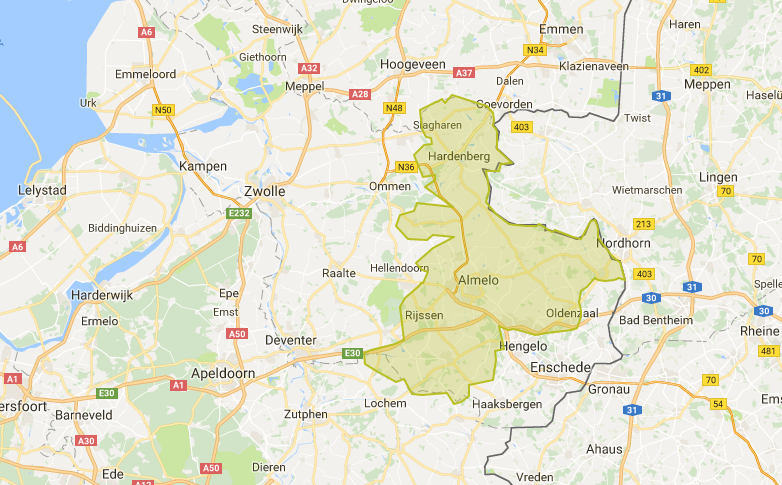
\includegraphics[width=.75\textwidth]{./figures/introduction/cogas_area.png}
\caption{The area Cogas has gas pipelines in.}
\label{fig:intro:cogas-area}
\end{figure}


